

% --------------------------------------------------------------

% This is all preamble stuff that you don't have to worry about.

% Head down to where it says "Start here"

% --------------------------------------------------------------



\documentclass[titlepage]{article}

\usepackage[margin=1in]{geometry} 
\usepackage{amsmath,amsthm,amssymb,scrextend,mathtools,siunitx, cancel, bm, xfrac, esint}
\usepackage{mdframed}
\usepackage{csquotes}
\usepackage{tabto}
\usepackage{tcolorbox}
\usepackage{tikz}
\edef\restoreparindent{\parindent=\the\parindent\relax}
\usepackage{parskip}
\restoreparindent

\usepackage{parskip,caption,gensymb}
\usepackage{graphicx,wrapfig,booktabs,multirow}
\usepackage{multicol}
\usepackage{placeins}
\graphicspath{./}
\usepackage{url}
\usepackage[table,xcdraw,dvipsnames]{}
\usepackage{fancyhdr,color,soul}
\usepackage{tikz}
\usepackage{textgreek}
\usepackage[dvipsnames]{}
\usepackage{float}

\renewcommand{\baselinestretch}{1.5} %this is your line spacing, current at, you guessed it! 1.5
\pagestyle{fancy}


\usepackage[hidelinks]{hyperref} %remove [hidelinks] and all links will have box surrounding
\usepackage{changepage}

\usepackage{color}

\usepackage{listings}
\usepackage{xcolor}

\definecolor{codegreen}{rgb}{0,0.6,0}
\definecolor{codegray}{rgb}{0.5,0.5,0.5}
\definecolor{codepurple}{rgb}{0.58,0,0.82}
\definecolor{backcolour}{rgb}{0.95,0.95,0.92}
\definecolor{quotecolor}{rgb}{211,211,211}

\lstdefinestyle{code}{
	backgroundcolor=\color{backcolour},   
	commentstyle=\color{codegreen},
	keywordstyle=\color{magenta},
	numberstyle=\tiny\color{codegray},
	stringstyle=\color{codepurple},
	basicstyle=\ttfamily\scriptsize,
	breakatwhitespace=false,         
	breaklines=true,                 
	captionpos=t,                    
	keepspaces=true,                 
	numbers=left,                    
	numbersep=5pt,                  
	showspaces=false,                
	showstringspaces=false,
	showtabs=false,                  
	tabsize=2
}
\lstset{style=code}

\lstdefinelanguage{ez80asm}{
	morekeywords={ld,lea,add,push,pop,lddr,ret},
	sensitive=false,
	morecomment=[l]{;},
	morestring=[b]",
}


% if you want to define a new color use this format: {name}{RBG}{R, G, B values}
%\definecolor{teal}{RGB}{0, 128, 128 } 
\definecolor{ltgray}{gray}{0.9}

\global\mdfdefinestyle{exampledefault}{%
	linecolor=white,linewidth=3pt,%
	backgroundcolor=ltgray,
	leftmargin=1cm,rightmargin=1cm
}

\newcommand*{\hamil}{\hat{\mathcal{H}}}


\newcommand{\N}{\mathbb{N}}

\newcommand{\Z}{\mathbb{Z}}

\newcommand{\I}{\mathbb{I}}

\newcommand{\R}{\mathbb{R}}

\newcommand{\Q}{\mathbb{Q}}

\renewcommand{\qed}{}

\let\newproof\proof



\renewenvironment{proof}{\begin{addmargin}[2em]{2em}\begin{newproof}}{\end{newproof}\end{addmargin}\qed}
% \newcommand{\expl}[1]{\text{\hfill[#1]}$}

\newenvironment{theorem}[2][Theorem]{\begin{trivlist}
		
		\item[\hskip \labelsep {\bfseries #1}\hskip \labelsep {\bfseries #2.}]}{\end{trivlist}}
	

\newenvironment{lemma}[2][Lemma]{\begin{trivlist}
		
		\item[\hskip \labelsep {\bfseries #1}\hskip \labelsep {\bfseries #2.}]}{\end{trivlist}}

\newenvironment{problem}[2][Problem]{\begin{trivlist}
		
		\item[\hskip \labelsep {\bfseries #1}\hskip \labelsep {\bfseries #2.}]}{\end{trivlist}}

\newenvironment{exercise}[2][Exercise]{\begin{trivlist}
		
		\item[\hskip \labelsep {\bfseries #1}\hskip \labelsep {\bfseries #2.}]}{\end{trivlist}}

\newenvironment{reflection}[2][Reflection]{\begin{trivlist}
		
		\item[\hskip \labelsep {\bfseries #1}\hskip \labelsep {\bfseries #2.}]}{\end{trivlist}}

\newenvironment{proposition}[2][Proposition]{\begin{trivlist}
		
		\item[\hskip \labelsep {\bfseries #1}\hskip \labelsep {\bfseries #2.}]}{\end{trivlist}}

\newenvironment{corollary}[2][Corollary]{\begin{trivlist}
		
		\item[\hskip \labelsep {\bfseries #1}\hskip \labelsep {\bfseries #2.}]}{\end{trivlist}}


\mdfdefinestyle{function}{%
	backgroundcolor=Tan!10,%
	linecolor=Tan,%
	linewidth=1pt,%
	leftmargin=0.1cm,%
	rightmargin=0.1cm,%
	roundcorner=10pt,%
	frametitlebackgroundcolor=Tan,%
}

\mdfdefinestyle{warning}{%
	linecolor=red,%
	linewidth=3pt,%
	leftmargin=-0.2cm,%
	rightmargin=-0.2cm,%
	skipbelow=0,%
	skipabove=0,%
	topline=false,%
	bottomline=false,%
	rightline=false%
}

\mdfdefinestyle{note}{%
	linecolor=YellowOrange,%
	linewidth=3pt,%
	leftmargin=-0.2cm,%
	rightmargin=-0.2cm,%
	skipbelow=0,%
	skipabove=0,%
	topline=false,%
	bottomline=false,%
	rightline=false%
}

\newtcolorbox{newquote}{
	fontupper=\normalsize\itshape,
	fontlower=\footnotesize,
	colframe=gray!50,
	boxrule=0.1pt,
	colback=gray!25
}
\setlength{\parindent}{0pt}

% --------------------------------------------------------------

%                         Start here

% --------------------------------------------------------------



%\lhead{left}

%\chead{center}

%\rhead{Right}

%If you uncomment any/all of the above, you can set your own headers, uncommenting one will remove the auto headers in place (section and subsection) 


\makeatletter\@enumdepth1\makeatother

\makeatletter
\def\@Aboxed#1&#2&#3\ENDDNE{%
	\ifnum0=`{}\fi \setbox \z@
	\hbox{$\displaystyle#1{}\m@th$\kern\fboxsep \kern\fboxrule }%
	\edef\@tempa {\kern  \wd\z@ &\kern -\the\wd\z@ \fboxsep
		\the\fboxsep \fboxrule \the\fboxrule }\@tempa 
	\fcolorbox{white}{ltgray}{$\displaystyle #1#2$}% changed
}
\makeatother

\begin{document}
	
			\begin{titlepage}
			\begin{center}
				\vspace*{2in}
				{\Large\textbf{CryptX}}
				\\\rule{.5\linewidth}{4px}\\
				{\huge\textbf{Industry-Standard\\Cryptography\\on the\\\vspace{4mm}TI-84+ CE}}
				\\\rule{.5\linewidth}{4px}\\\vspace{4mm}
				{\large\textit{Version 10.0}}\\\vspace{4mm}{\Large Analysis \& Extended Information}\\
				\vspace*{2in}
				by Anthony Cagliano
			\end{center}
		\end{titlepage}
	\setcounter{secnumdepth}{2}
	\setcounter{tocdepth}{2}
	\tableofcontents
	\begin{center}
		\rule{1\linewidth}{2px}
	\end{center}
	\section*{Foreword}
		Despite being developed for an unconventional platform, CryptX implements some of the most secure encryption in use today with an API capable of generating secure keys and salts, as well as constructing secure channels of communication between the device and a host computer or server. The library facilitates obfuscation and integrity of transmitted information between two endpoints, and also allows for authentication and identity verification between said endpoints. This document is a technical descriptor, providing details relevant to the construction of algorithms within CryptX that were built from the ground up, as well as providing details of hardening measures taken to ensure the library is as secure as possible. This document is provided such that platform-specific components of the library are able to be analyzed and peer-reviewed. For basic help with using the library, including overviews of defines, macros, and functions, consult the separate \textit{CryptX Quick Reference} document, which is more geared towards general library documentation.
		
		I would like to offer a special thanks to the members of the Cemetech programming community whose support and assistance has made the continuing development of this library possible. Not only have a few members been active contributors to this project's code-base, but many others have contributed to discussions on SAX and Discord about entropy, math and proofs, and methods of hardening the library against attack.
	\newpage %starts intro on next page, remove and it'll start just under contents
	
	\section{CSRNG Construction \& Analysis}
	\label{ssec:csprng}
		\subsection{Construction Overview}
			The \texttt{CSRNG} is the most platform-dependent part of this code, and consequentially the part of it the most work was done on. The first question to answer in the quest to devise one was does the TI-84+ CE produce randomness, and if so, how does this differ by hardware revision. The calculator is unlike a computer in that it lacks many of the dynamic sources of entropy that go into generating randomness for those platforms. While in the algorithm-development process, I posted on \underline{\href{https://cemetech.net}{Cemetech}} seeking information about possible sources of randomness on the TI-84+ CE. I was soon informed about the viability and functionality of hardware "bus noise" by Cemetech user \textit{Zeroko}.
			\begin{newquote}
				SRAM has a pair of bitlines for each bit of each column address, which are connected to a circuit that tries to make them both be charged to an equal, high level before reading from a memory cell (which partially discharges one of the two) and to a sense amplifier (basically a comparator) to read the resulting state afterward. (There may also be another level of gating between the bitlines and the comparators, but that does not strongly affect the dynamics.) In the unmapped space, there are no memory cells, so the controller equalizes the bitlines however well it does, then does nothing (there being no memory cell to discharge them), then senses which bitline is at a higher level. For some column addresses, this will be heavily biased one way or the other because the pre-charge transistors on the bitlines are too different, while for others, it will be less biased because they are more similar. 
				\tcblower
				Cemetech user "Zeroko", \underline{\href{https://www.cemetech.net/forum/viewtopic.php?p=293079}{Producing Crypto-Safe Randomness on the TI-84+ CE}}, May 2021
			\end{newquote}
			This is the mechanism that drives the hardware-based RNG. Based on this information and on the technical information available about this behavior across various revisions of the TI-84+ CE, I constructed an algorithm that polls each bit of every byte in this address space looking for the bit with the least bias (out of N bit reads, the bit was set closest to 50\% of the time). The maximum leeway in the source bit is a bias of up to 75\% in either direction, but the algorithm will always favor the least biased bit. The most optimal byte is set internally, and is unable to be modified by the user. This allows for use of the same code regardless of hardware or software revision. Should a bit of sufficient entropy not be found the function will return \texttt{NULL}, and calls to the other \texttt{CSRNG} functions will return either \texttt{0} or \texttt{NULL}.
	
			The HWRNG reserves an entropy pool 119 bytes large in the device's accelerated RAM (to make the generator faster). To generate a random number, each byte in the entropy pool is updated by reading from the selected source byte (the byte containing the bit with the most entropy). The entire pool is then passed through the SHA-256 cryptographic hash, generating a 32-byte digest. That hash is broken into 8-byte blocks, each byte of which is xored together to produce a single byte. The result is a 4-byte compression of the 119 byte entropy pool.
			
		\subsection{Correlation in the Bit Stream}
		
		Due to the nature of the CE hardware, there is a measurable correlation in the values of floating bits within unmapped memory. This correlation varies depending on the sample size, but would measurably reduce the entropy of the system. While specific numbers on the degree of correlation are, as of yet, unavailable, we do know that there are higher amounts of correlation in the initial reads which decreases after a certain number of reads. To combat this, the entropy gathering function was rewritten with direction from Zeroko.
		\begin{newquote}
		Another source of non-randomness distinct from the bias is that the bitlines act like capacitors, so precharging only moves their voltage toward the desired level rather than reaching it. This results in a correlation between reads, with the correlation getting weaker with a longer time interval between them and with more intervening reads performed. This is why we cannot just use a von Neumann extractor (which only de-biases) and instead have to do something like XORing many consecutive bits together (which does not fully remove the bias and correlation but can lower it to an undetectable level). 
		\tcblower
		Cemetech user "Zeroko", \underline{\href{https://www.cemetech.net/forum/viewtopic.php?p=293079}{Producing Crypto-Safe Randomness on the TI-84+ CE}}, May 2021
		\end{newquote}
		After some discussion it was agreed that making each byte in the entropy pool a composite of seven (7) distinct reads from the source byte XORed together would yield acceptable results with entropy negligibly less than what is computed in Section 1.3.
		
		\subsection{Proof of Cryptographic Security}
			In order to be secure (at least on paper), a PRNG has to pass 2 distinct additional unpredictability assessments in addition to the requirement that it also pass general statistical randomness tests. The two additional tests are the \textbf{next-bit test} and the \textbf{state compromise test}.
				\begin{newquote}
					Given the prior output of the PRNG (bits 0 -$>$ i), the next bit (i+1) of the output cannot be predicted by a polynomial-time statistical test with a probability non-negligibly greater than 50\%.
					\tcblower
					\textbf{Next-Bit Test}
			\end{newquote}
			\begin{newquote} 
					An adversary gaining knowledge of the initial state of the PRNG does not gain any information about its output.
					\tcblower
					\textbf{State Compromise Test}
			\end{newquote}
			To solve the next-bit test, I'll make a few assumptions. Firstly, a secure PRNG must pass all statistical tests. A cryptographic hash, like SHA-256, produces output that satisfies this constraint, regardless of the entropy of its input. Second, each output of the PRNG is a 32-bit or 4 byte unsigned integer, meaning we need at least 32 bits of entropy to generate such an integer. Observe the computation below that plugs the worst-case bias in the source byte into the Shannon entropy formula to calculate the available entropy across the 119 bytes of the entropy pool.
			\begin{mdframed}[style=exampledefault]
				\begin{proof}
				\textbf{Entropy for Worst-Case Byte Selection}
				
				The byte selected for use by the CSRNG will have at least one bit with a maximum bias of 75\% (± 25\% deviation from 50/50), with the rest of the byte likely having a much higher bias. To this end, we will assume 100\% bias, or 0 entropy, for them. The entropy of the 75/25 bit can be represented as the set of probabilities {.75, .25}, which can be applied to the equation for Shannon entropy:
		\[
			H(bit)=\sum_{i=1}^nP(i)\log_2\frac{1}{P(i)}
		\]
			Where $n$ is the length of the set of probabilities and
			$P(i)$ is the probability of the $i$-th element in the set
		\[
			H(bit)_{min}=0.750\log_2\frac{1}{0.750}+0.250\log_2\frac{1}{0.250}=0.811
		\]
		%	\[
		%	\Aboxed{E_{min}=0.811}
		%	\]
			Assuming that this is the entropy of the bit selected, and also assuming that the rest of the byte in question has minimal entropy (whether this is true or not depends on what byte we are selecting. Sometimes there is some entropy in other bits of the byte, other times the bit values are predictable), the entropy for the entire byte (worst-case) can be calculated like so:
		\[
			H(byte) = 0.811 + (7*0) = 0.811			
		\]
			The entropy pool consists of 119 bytes, so to compute the available entropy we multiply the entropy per byte by the size of the pool.
		\[
			H(pool)_{min}(119)=0.811\times119.0=96.51
		\]
		%	\[
		%	\Aboxed{E_{min}(128)=103.8}
		%	\]
	\end{proof}
	\end{mdframed}
	This means we have 96.51 bits of entropy per 32-bit number at minimum, more than double what is needed. Because the available entropy exceeds the bit-width of the number we are generating, I assert that the probability of \texttt{r <-- \{0,1\}} is within a negligible deviation, \textepsilon, from $\dfrac{1}{2}$ for all bits in the 32-bit number. This would also mean that the advantage of an adversary attempting to differentiate the output of this CSRNG from a uniform random distribution would also be negligible.
	
	Having proved sufficient entropy in the input, I assert that the output of the generator satisfies all algorithmic constraints for cryptographic security and will now move onto the second test, state compromise. Each output of the generator is based on a freshly-constructed entropy pool, meaning that there is no computational relationship between subsequent invocations of the CSRNG. This means that there is no "initial state" of the generator (apart from what byte we are reading entropy from, and leaking that reveals nothing of value), and even the leaking of a prior state of the generator will not compromise the next output. Thus, I assert that this generator also passes the state compromise test, and is thus safe for use as a cryptographic RNG.
	
	Note that these proofs only apply to physical hardware (an actual TI-84+ CE), not to emulators. Due to their inability to reproduce the behavior of the unmapped region, they implement a deterministic RNG to create the illusion of randomness for that range of memory. This yields statistical randomness with an obscurity factor due to how HASHLIB selects the source, but the randomness is still not cryptographically secure. Bear this in mind when using HASHLIB from CEmu.
	
	\section{Side-Channel Analysis}
		HASHLIB has an unknown level of resistance to side-channel analysis. The TI-84+ CE is not a device constructed with hardware security in mind, despite TI repeatedly trying to improve security by taking actions that have nothing to do with security. One such example was disabling native assembly code execution to fix a bug that had already been resolved just to appease a bunch of bureaucrats who were well-informed enough to know the bug existed, but not well-informed enough to know that it had already been patched. This led to greater efforts at breaching and exposing ways to execute code anyway--and not everyone who now has access to that exploit would have the same benevolent intent that myself and the rest of the TI programming community does. Pro-tip: allowing non-field experts to control policy is a really good way to get your policy wrong. You don't see archaeologists controlling cybersecurity standards. A bit of advice for TI if any of you wind up seeing this-- You don't nuke an entire feature set to deal with one specific, unrelated, vulnerability. It's more to your advantage to re-enable assembly execution and rethink exam security specifically.
		
		With that rant over, let's circle back to the subject matter at hand--HASHLIB's resistance to side-channel analysis. There are very limited ways in which a device designed to be plugged into a computer and memory-mapped can be protected against being plugged into a computer and memory-mapped. That being said, I took some actions that could reasonably be taken without slowing down the library's functions to harden it against these types of attacks.
		
		\subsection{Timing Analysis Protection}
			One of the first considerations in this library was resistance to timing analysis. While I have not as of the time of this writing evaluated the ported functions, all functions written from scratch for this platform had this form of hardness in mind. The buffer comparison function and the modular exponentiation functions are two examples of this. Over time more of the library will be reviewed and, where necessary, the same considerations will be extended to those functions as well, where necessary.
		
		\subsection{Buffer Leak Protection}
			Another consideration taken within HASHLIB was to avoid leaving residual computational data in the stack frame after a function that performs data transformations completes. For this reason, some code was written that purges the stack frame and we call that code in most of the user-facing encryptor functions before returning control to the caller. For reference, the code used to accomplish this is:
			\lstinputlisting[style=code,language=ez80asm,caption={stack purging code by Zeroko}]{code/stack_clear.asm}
		\subsection{Memory-Mapping Protection}
		  	After resolving buffer leaks, our attention turned to thwarting attempts to map the device's memory while HASHLIB is running to glean information about the encryption or decryption. While there is sufficient difficulty in achieving this in a device designed to be used in that manner in other contexts, I believe the solution arrived at is sufficient.
		  	
		  	It is the system interrupt that makes it possible for the operating system to handle activity on the USB port, and disabling said interrupts would severely hamper attempts to read HASHLIB's state by preventing the system from responding to USB transfers. For this reason, some code was written that disables interrupts in all functions where data is being encrypted or decrypted, saving their state to SMC, and restoring that state afterwards. While there are many variations of this code that operate in slightly different ways depending on when they are called, here is the basic version of it, for reference:
		  	\lstinputlisting[style=code,language=ez80asm,caption={disable interrupts code by beckadamtheinventor}]{code/disable_interrupts.asm}
		  	
	\section{Algorithmic Security}
		\subsection{CPA Resistance}
			CPA is an acronym for \textit{chosen plaintext attack}, a type of attack against an encryption algorithm that involves an attacker gaining information about the secrets (keys) used for encryption by requesting encryptions of arbitrary plaintexts. The simplest way to explain this is to liken it to a system of multi-variable algebraic equations. With only one equation in the system it is unsolvable but if you begin to add more equations, suddenly it becomes possible to solve for and even eliminate variables. In a similar manner an encryption system with \textit{perfect secrecy} can still be completely broken by a chosen plaintext attack, although the methods of doing so are vastly more complicated than merely "solving a system of equations".
			
			All of the encryption functions in HASHLIB facilitate CPA security by allowing for the inclusion of a random oracle in the encryption. A random oracle simply means a string of unpredictable random bytes. In other places you may also hear or read the terms \textit{salt} or \textit{nonce}. These mean the same thing. In AES, as illustrated in the image on the left below, the randomness is included through the use of an \textit{initialization vector}, a buffer equal in size to the AES block size, filled with random data. In RSA, the randomness is added via the optimal asymmetric encryption padding scheme (OAEP), illustrated to the right, which xors the entire message with a salt using a Feistel network.\\
			\fbox{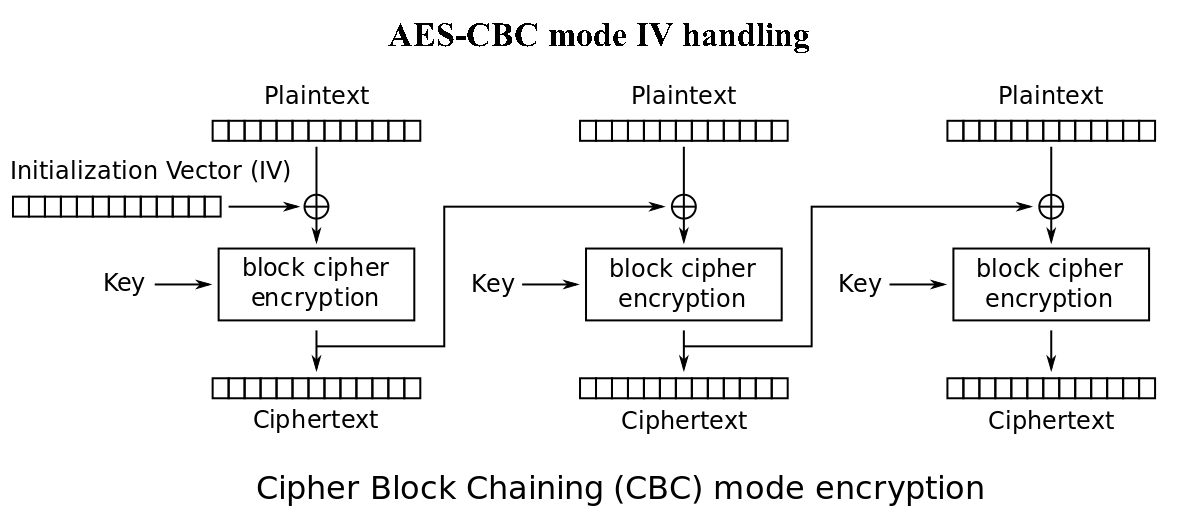
\includegraphics[width=0.60\textwidth]{imgs/cbc_mode.png}}
			\fbox{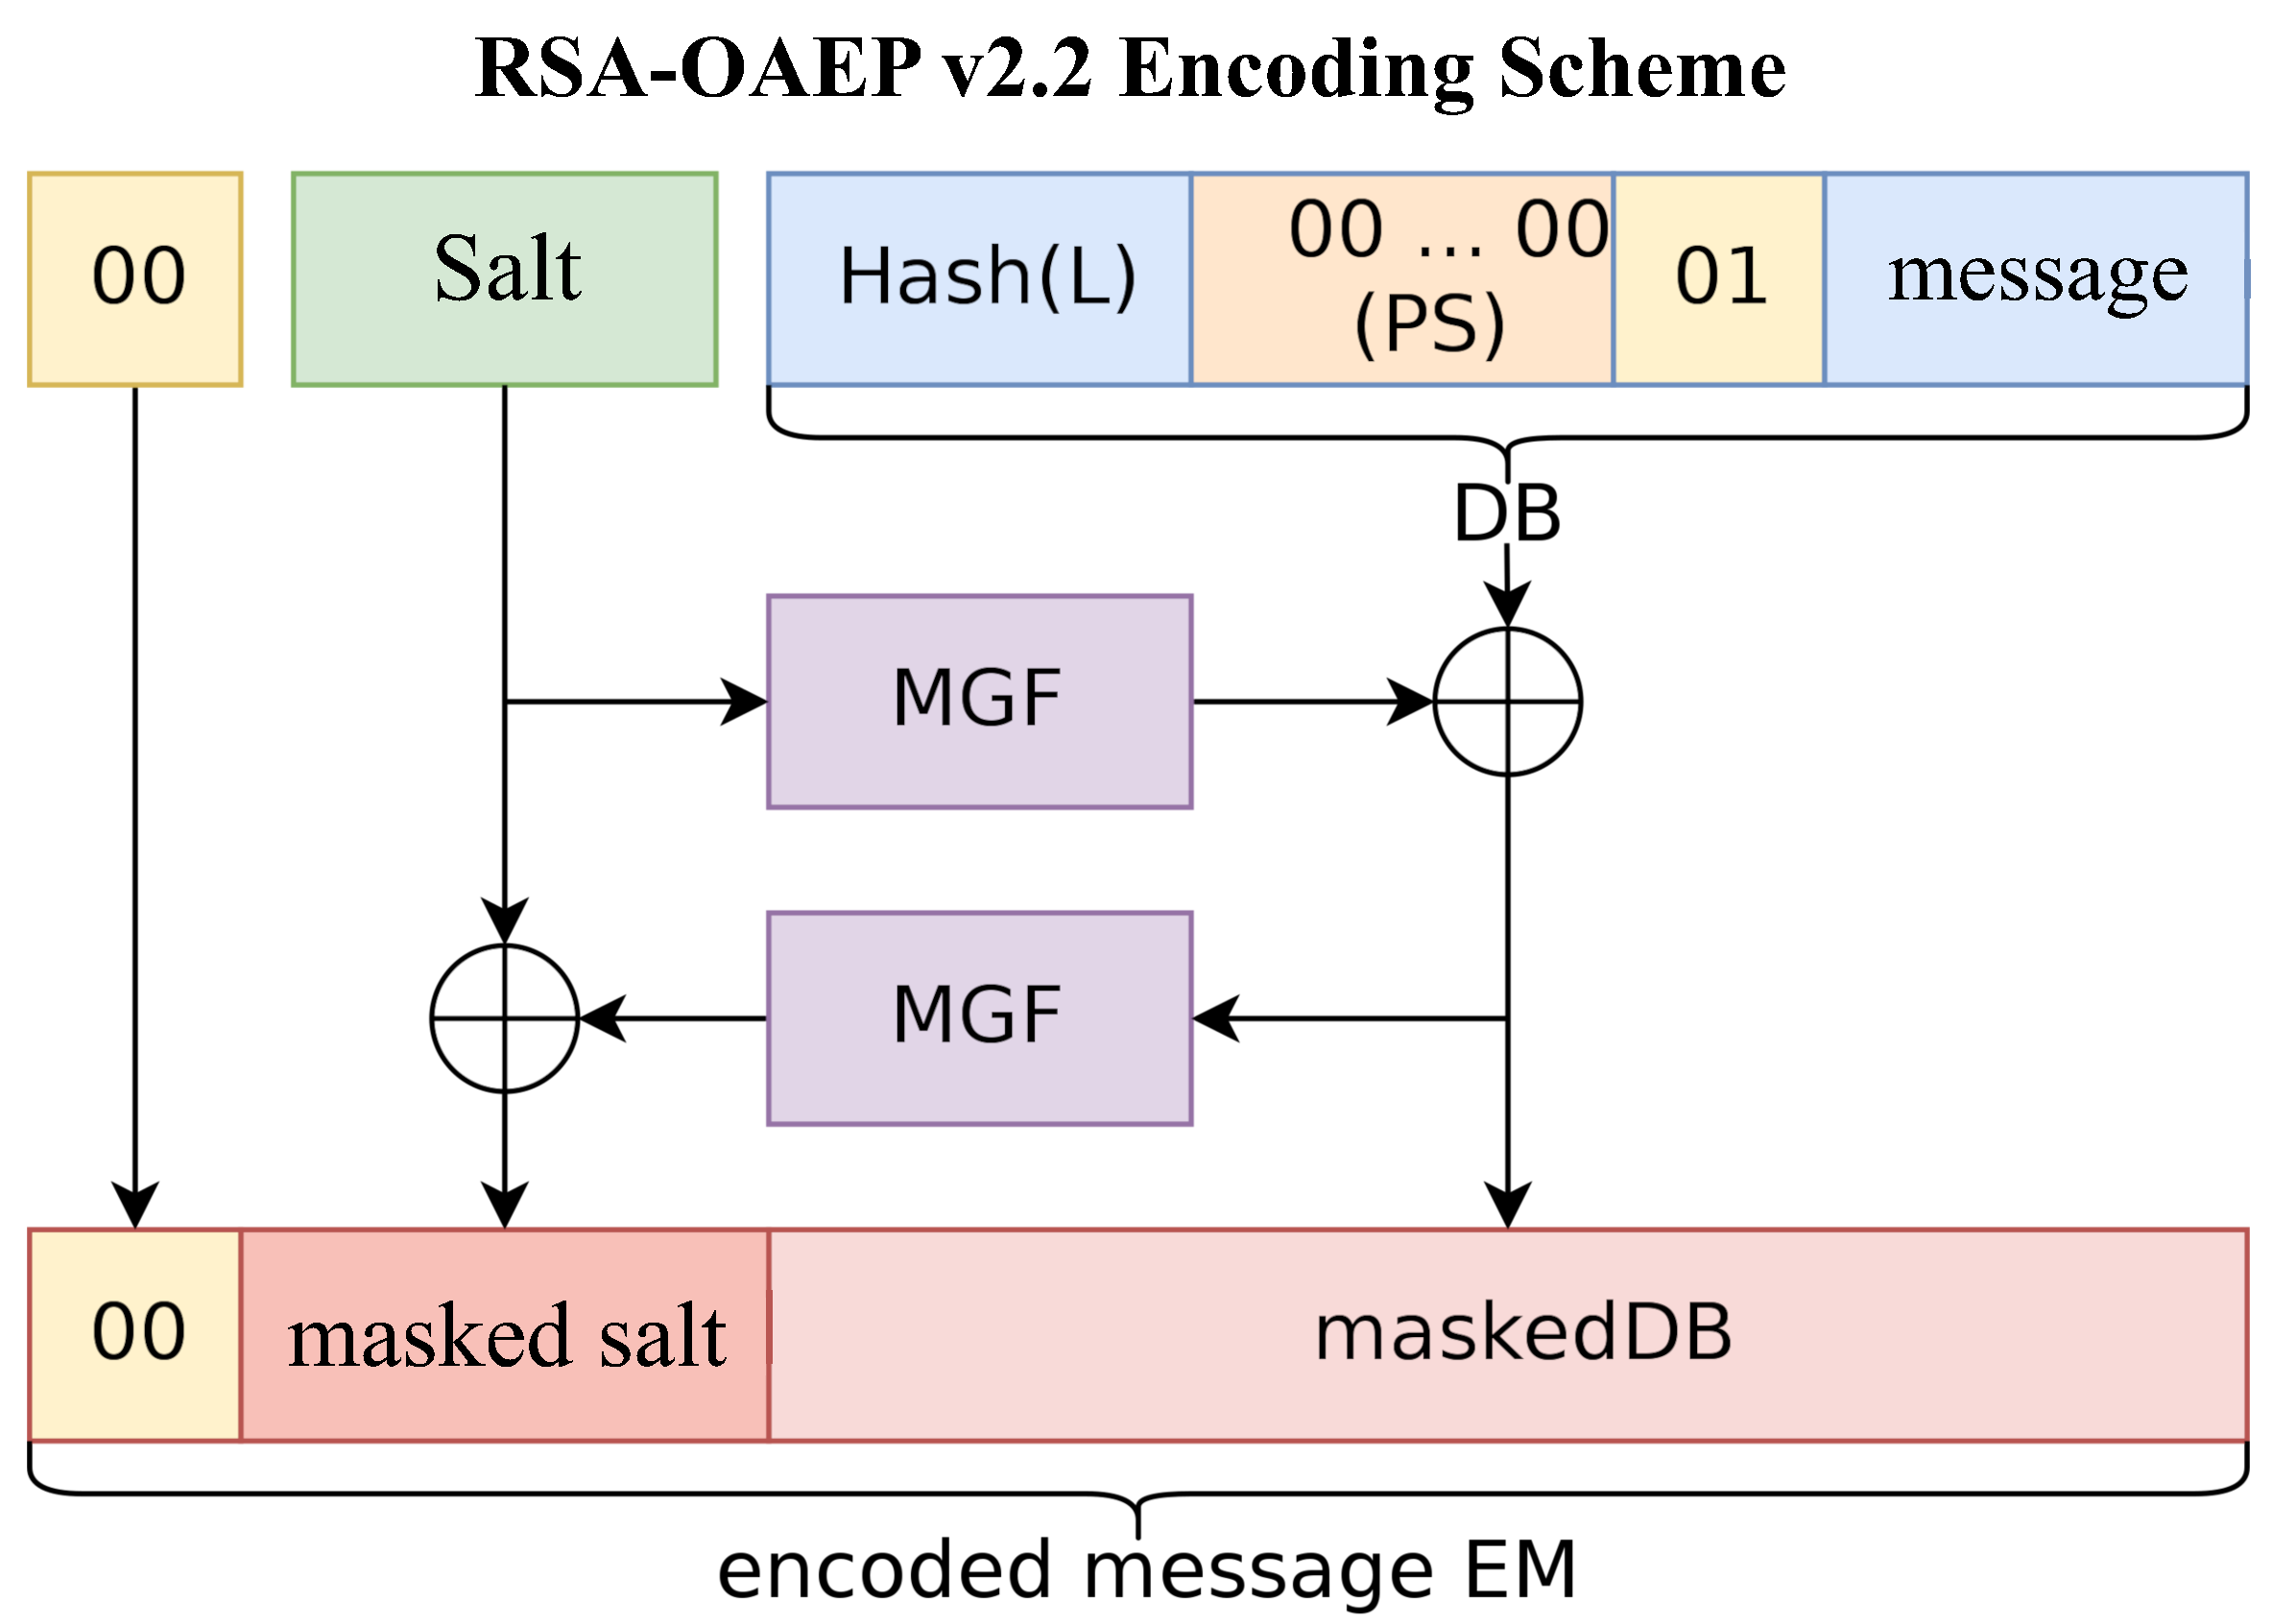
\includegraphics[width=0.40\textwidth]{imgs/oaep.png}}
			\textit{Images above sourced from Wikipedia and verified for correctness. CBC mode is not the only cipher mode that is CPA secure, it is just used as an example.}
		\subsection{CCA Resistance}
			CCA is an acronym for \textit{chosen ciphertext attack}, a type of attack against an encryption algorithm that involves an attacker gaining information about the secrets (keys) used for encryption by requesting decryptions of arbitrary ciphertexts. The objective of the attacker is the same, to "solve" for the encryption secret by requesting decryptions of chosen ciphertexts until characters of the key are revealed. However, because CCA works backwards to CPA, the random oracle that provides CPA security does not help us here. CCA security requires some form of authentication integrated with the encryption.
			
			Typically \textit{authenticated encryption} is accomplished in one of two ways: (1) using a specialized encryption cipher mode that produces an authentication tag in parallel with the encryption and a specialized decryption cipher mode that can validate this authentication tag while decrypting, or (2) appending a hash or keyed hash to the message that is validated BEFORE decryping the message. The former method is generally considered to be more secure but is also more computationally intensive. For this reason, HASHLIB provides an API for the latter. A series of rules for properly constructing an authenticated encryption scheme using the included hash and hmac implementations can be found in \textit{HASHLIB Quick Reference, Section 2.8}. It will be on the user to follow the rules properly, or their implementation may be insecure.
	\newpage
	\section{Conclusion}
		In summation, HASHLIB is a work-in-progress and sees regular updates that add resistance to various forms of attack. While its algorithmic security is solid if implemented properly, hardware-based attack is harder to defend against due to the nature of the hardware. Thus far, some significant actions have been taken to secure the library against hardware-based attack and HASHLIB's code is publicly available on forums frequented by others familiar with the CE's hardware and is under continuous peer-review with the aim of continually improving the library's security profile.
		
		If you have any questions about the proper usage of HASHLIB in your programs, any of its functionality, algorithms, etc, please do not hesitate to contact me on Discord at \texttt{acagliano\#3685}. I would rather you ask questions than implement security improperly and risk compromising your implementation.
		
		{\color{red}\textbf{Please update to new stable releases of HASHLIB as soon as they become available and update any software you are developing to use the latest versions of HASHLIB as soon as you are able. At this stage in HASHLIB's development, updates are security enhancements, not major feature additions.}}

		\section{References}
			[1] \href{https://github.com/B-Con/crypto-algorithms/}{{\underline{https://github.com/B-Con/crypto-algorithms}}\label{bcon}}
			\tabto{5mm}source of AES and SHA-256 initial algorithms ported to platform\newline
			\tabto{5mm}SHA-256 later rewritten in ez80 Assembly by beckadamtheinventor\newline
			\newline
			[2] \href{https://www.cemetech.net/forum/viewtopic.php?p=293090#293090}{{\underline{ https://www.cemetech.net/forum/viewtopic.php?p=293090\#293090}}\label{cemetech}}
			\tabto{5mm}source of information on randomness on the TI-84+ CE\newline
			\newline
			[3] \href{https://en.wikipedia.org/wiki/Cryptographically-secure_pseudorandom_number_generator}{{\underline{ https://en.wikipedia.org/wiki/Cryptographically-secure\_pseudorandom\_number\_generator}}\label{csprng}}
			\tabto{5mm}information on constructing a secure PRNG\newline
			\newline
			[5] \href{https://datatracker.ietf.org/doc/html/rfc8017}{{\underline{https://datatracker.ietf.org/doc/html/rfc8017}}\label{oaep}}
			\tabto{5mm}guidance on implementing RSA-OAEP and RSA-PSS padding schemes\newline
			\newline
			[6] \href{https://datatracker.ietf.org/doc/html/rfc4868}{{\underline{https://datatracker.ietf.org/doc/html/rfc4868}}\label{hmac}}
			\tabto{5mm}guidance on implementing SHA-256 HMAC\newline
\end{document} 






